\documentclass[unicode]{beamer}

\mode<presentation>
{
	\usetheme{Warsaw}
%	\setbeamertemplate{headline}{}
%	\setbeamertemplate{footline}{}
}

\usepackage[utf8]{inputenc}
\usepackage[T2A]{fontenc}
\usepackage{amssymb, amsmath, hyperref}
\usepackage[main=russian,english]{babel}

\title{Автоматическая транскрипция музыки (AMT)}
\author{Сергей Синяк}
\date{Минск, 2017}

\begin{document}

\begin{frame}
	\titlepage
\end{frame}

\section{Характеристика работы}
\begin{frame}
  За время работы над дипломом были рассмотрены различные подходы
  для решения задачи автоматической транскрипции музыки.
  Они включают преобразование фурье, константное Q преобразование,
  NMF и машинное обучение.
  Стоит отметить относительный успех применения нейронных сетей
  на базе датасета MAPS. Ведь только здесь удалось вернуться
  к исходной постановке задачи, а именно когда
  дан набор шаблонов наигранных нот и требуется распознать
  произвольную нотную последовательность исполненную на том же
  инструменте.
\end{frame}

\section{Содержание}

\begin{frame}
   Отметим план/содержание работы в экспериментах с нейронными сетями
  \begin{enumerate}
    \item Подготовка датасета
    \item Обработка данных и формирование тренировочной и тестовой выборок.
    \item Определение функции потерь и целевой функции точности.
    \item Эксперименты с архитектурой нейронной сети, её обучение и
      валидация
    \item Визуализация результата работы
  \end{enumerate}
\end{frame}

\section{Нейронная сеть}

\begin{frame}
  Нейронная сеть представляет собой граф вычислений, в котором вершины
  отождествляют собой монотонные функции активации, а дуги указывают
  направления её передачи. Отдельно выделяют входной слой --- вершины
  в которые передются входные данные, обычно одно число на одну вершину
  входного слоя. И выходной слой --- это вершины, активации которых используются
  для трактования работы системы и обычно обрабатываются для порождения
  желаемого распределения значений в соотвествии с целевой задачей.
  Все остальные вершины определеют внутренние слои.
\end{frame}

\begin{frame}
  Полносвязным слоем называется преобразование следующего вида:
  \[
    h_{l + 1} = g(W_l h_l + b_l),
  \]
  где $h_l$ и $h_{l + 1}$ это значения активации вершин $l$-ого и  $l+1$-ого слоев,
  а $g(W_l h_l + b_l)$ задаёт их функциональную связь.
  $W_l$ называется матрицей весов дуг
  между слоями $h_l$ и $h_{l + 1}$, $b_l$~--- это смещение. Как видим
  в аргумент функции $g$ поступает некоторое афинное преобразование
  от параметров $h_l$.
\end{frame}

\begin{frame}
  Для добавления нелинейности, функцию $g$ обычно выбирают нелинейной.
  Классической является сигмоид:
  \[
    g(x) = \sigma (x) = \frac{1}{1 + e^{-x}}
  \]
  Обычно g(x) обладает свойствами:
  \[
    0 \leq  g(x) \leq 1,
  \]
  но необязательно.
\end{frame}

\begin{frame}
  Формально для нейронной сети можно задать начальные значения всем параметрам,
  а именно весам $W_l$ и $b_l$, также выбрать функции активации $g$.
  Затем согласно некоторой функции потерь,
  пр. $m(Y_{pred}, Y) = 1.0 - F(Y_{pred}, Y)$
  решить задачу минимизации:
  \[
    \text{ Найти $\hat f$, что } \forall \; X=\{{x_0^t}_j\}, Y=\{{y_0^t}_j\}:
  \]
  \[
    \hat f = \underset{f}{\text{argmin}}(1 - F(f(X), Y))
  \]
\end{frame}

\begin{frame}
  Архитектура нейронной сети была простейшая и состояла
  из одного скрытого полносвязного слоя до 2048 вершин,
  и последующего полносвязного слоя на 88 вершин для классификации
  и выдачи активаций соотвествующих MIDI частот.
\end{frame}

\begin{frame}
  Из результатов хочется отметить, что используя суммарный датасет на 1.6
  миллиона фреймов, нейронная сеть за 8 часов на машине с процессором
  2x1.6GHz обучилась до значения функции потерь на базе F-меры равного 0.28.
\end{frame}

\begin{frame}
\begin{figure}
  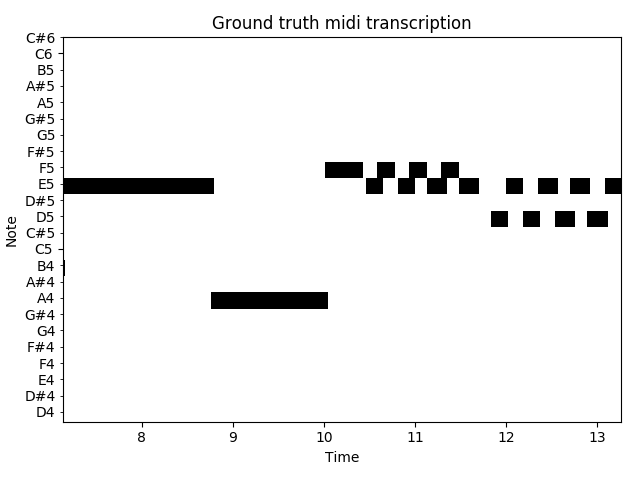
\includegraphics[scale=.6]{res/organ-note-groundtruth-zoomed-for-presentation.png}
\end{figure}
\end{frame}

\begin{frame}
\begin{figure}
  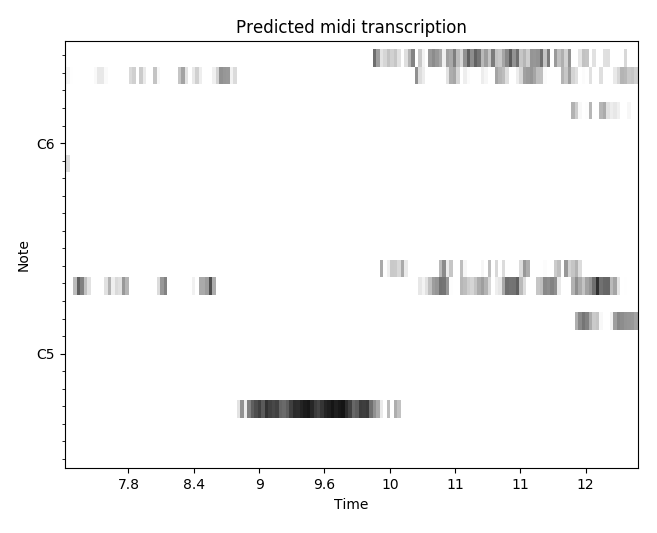
\includegraphics[scale=.6]{res/organ-overfit-028-acoustic-zoomed-for-presentation.png}
\end{figure}
\end{frame}

\begin{frame}
\begin{figure}
    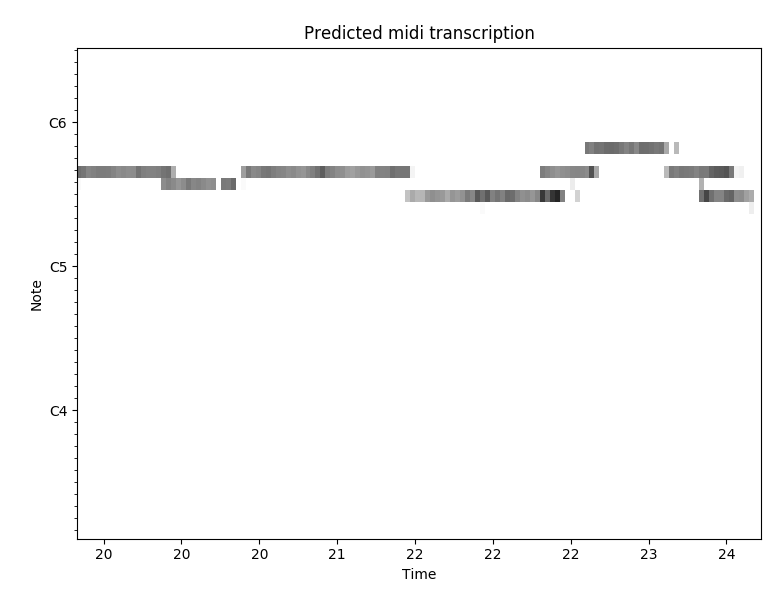
\includegraphics[scale=.5]
      {res/daj-ci-boze-dobranoc-overfit-028-acoustic-zoomed-for-presentation.png}
\end{figure}
\end{frame}

\section{Заключение}

\begin{frame}
  \center{Спасибо за внимание!}
\end{frame}

\end{document}
